\chapter{Integration of IO Channels in MIDG2}
\label{cha:sys_arch}

MIDG2\footnote{\url{https://github.com/tcew/MIDG2}} is used as the target
application in this thesis to evaluate the benefits of using IO channels.
MIDG2 application uses the \ac{DG} method to calculate the electric and magnetic
field values for objects as described in the chapter \ref{cha:Fundamentals}.
The thesis extends the MIDG2 \ac{MPI} FPGA version of the application introduced in the
section \label{sec:midge_mpi} which uses OpenCL kernels to
offload the performance critical calculations to the FPGA accelerators in a
distributed system and use MPI to communicate among the different instances of the
host application. The system scales over multiple nodes as discussed but
uses the \ac{MPI}+PCIe to communicate which have low bandwidth as shown in section
\ref{sec:top_eval}. To improve the bandwidth performance of the application,
the IO channels are proposed to be used. This chapter explains the changes
which are done to the OpenCL kernels and the host application in order to use
the QSFP Network Ports to build up topologies discussed in chapter
\ref{cha:topologies} to allow direct communication between the FPGAs to create a
\texttt{MIDG2 FPGA IO channels} design
and evaluate the benefits of the direct communication with the MIDG2 application.

\section{Kernel Structure with IO Channels}
\label{sec:struc_iochan}

The first set of changes done in the thesis to the \texttt{MIDG2 MPI FPGA} application
was to include the IO channels to exchange the shared data in a multiple FPGA system.
The IO channels are used to exchange the shared data between the FPGAs directly instead
of copying it first to global memory, which is read by the \texttt{Host application}
and then transferred using MPI. The prototypes developed for the topology's evaluation
serve as the basis to implement the support for IO channels in the OpenCL kernels for
the MIDG2 application. The main modification required to enable the OpenCL MIDG2
kernels to communicate via IO channels
was to remove the \texttt{partial\_get\_kernel} and replace it with two kernels
\texttt{partial\_send} and \texttt{partial\_recv}. The implementation of these kernels
is similar to the prototype \texttt{send} and \texttt{recv} kernels described in
section \ref{sec:proto_topo}. Two different set of kernels for the two topologies,
the \texttt{within node} and \texttt{fully connected} are developed. The \texttt{within node}
scales the application to two FPGAs and the \texttt{fully connected} to 4 FPGAs.

As explained in the section \ref{sec:midge_mpi_struc}, \texttt{partial\_get\_kernel} reads
the shared from the \texttt{g\_Q} memory and writes them back into another buffer
to coalesce the shared data. The new \texttt{partial\_send} and \texttt{partial\_recv}
split these operations and also perform the communication with the
other FPGA over the IO channels. The \texttt{partial\_send} kernel reads the
shared elements from the \texttt{g\_Q} buffer and sends the shared elements data
over a single or multiple external channel to other FPGA(s).
The \texttt{partial\_recv} receives the data from other FPGAs over the channels and
then stores it in \texttt{g\_partQ} buffer which is passed to the \texttt{SURFACE}
kernel for processing.

In the \texttt{within node} topology, the data is only exchanged between two nodes
which simplifies the channel assignment for the shared data. All the shared data is sent and received
to/from only one node using one or four channels. In the \texttt{fully connected} topology,
the communication is not straight forward. In a 4 node system, the shared elements are mapped
to different nodes. The \texttt{partial\_send} and \texttt{partial\_recv} kernels need this mapping
information at the runtime to transfer and receive data correctly to/from target node. The mapping information
for identifying the indexes to be read from the \texttt{g\_Q} is provided in another buffer
\texttt{g\_index}. \texttt{g\_index} contains the list of the indexes of the shared data
sorted by the target \ac{MPI} rank. \texttt{g\_index} was used in the \texttt{partial\_get\_kernel}
of the MIDG2 \ac{MPI} FPGA application to identify the shared data. For IO channels design along with
\texttt{g\_index}, additional information for mapping the indexes to specific target FPGA is
passed by using two parameters \texttt{start<x>} and \texttt{nout<x>} for each channel \texttt{x}.
In the \texttt{partial\_send} kernel, the \texttt{start<x>} specifies the start location within \texttt{g\_index}
and the \texttt{nout<x>} specifies the number of indexes to send for the channel \texttt{x}. In
\texttt{partial\_recv} the \texttt{start<x>} specifies the start index within the \texttt{g\_partQ}
and the \texttt{nout<x>} specifies number of index to receive for channel \texttt{x}. As each
channel is assigned to a specific FPGA node, \texttt{start<x>} and \texttt{nout<x>} map
the data for a target FPGA to the channel used to connect with the target FPGA.

With this information, The \texttt{partial\_send} is able to read data from \texttt{g\_Q}
for all channels simultaneously, and send them over the respective channel. Also, the \texttt{partial\_recv}
kernel is able to receive the data and write them into \texttt{g\_partQ} simultaneously. The first
version of the \texttt{partial\_send} and \texttt{partial\_recv} kernels used this information for
mapping the memories to channels but memory dependencies were reported in \texttt{partial\_recv} kernel by the Intel OpenCL FPGA compiler.
As the received data in the \texttt{partial\_recv} is written into the same \texttt{g\_partQ} buffer,
the Intel OpenCL compiler identified the multiple memory writes as interdependent and serialized the channel
read and memory writes as shown in Figure \ref{fig:serial_reads}.
\begin{figure}[ht]%
    \centering
    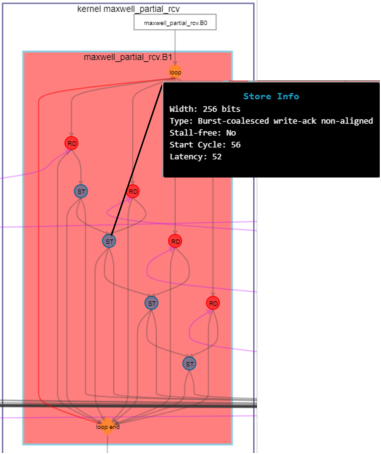
\includegraphics[width=0.45\textwidth]{images/serial_reads}
    \caption{Memory dependency resulting in serial channel reads in the \texttt{partial\_recv}
    for \texttt{fully connected} design}
    \label{fig:serial_reads}
\end{figure}
As the data from each channel is written
into different location in the buffer (different \texttt{start<x>} values), there is no
dependencies or overlaps the parallel writes would not create any memory corruption. The Intel OpenCL compiler
was unable to understand it from the existing structure and also there is no way to correctly specify this in the kernel code.
So, to resolve this issue, \texttt{g\_partQ} buffer was aliased into four
different names \texttt{g\_partQ[1-4]}. Each of the \texttt{g\_partQ<x>} buffer is used
for individual writes of the data received from channel \texttt{x} though they are initialized by the same
OpenCL buffer in the \texttt{Host application}. This change allowed
Intel OpenCL compiler to create a sequence with parallel writes to the \texttt{g\_partQ} buffer.


The addition of double buffer in MIDG2 \ac{MPI} FPGA allowed improving the execution of the kernels
by reducing the load on the \texttt{g\_Q} buffer and executing \texttt{RK} kernel immediately after completion
of computation for both shared and non-shared data separately. Though there was improvement,
\texttt{RK} still executed after the compute kernels which was not desirable. Further optimization
by introducing Intel OpenCL channels between \texttt{VOLUME/SURFACE} to \texttt{RK} to replace
\texttt{volrhsQ} and \texttt{surrhsQ} was possible but was not implemented before the start of the thesis.
So, this optimization to the kernel pipeline is introduced in this thesis as part of the IO channel implementation
which could help to improve the performance of the kernels marginally.
The OpenCL kernels implementation is updated to include internal channels to
communicate the right-hand side field values
from \texttt{VOLUME/SURFACE} to \texttt{RK} as shown in the kernel structure
in Figure \ref{fig:iochan_kernstruc}. Use of channels allows execution of all three
kernels simultaneously giving a deeper pipeline structure and improving the throughput
of the design by performing parallel computation in \texttt{VOLUME}, \texttt{SURFACE} and \texttt{RK} kernels.

\begin{figure}[ht]%
    \centering
    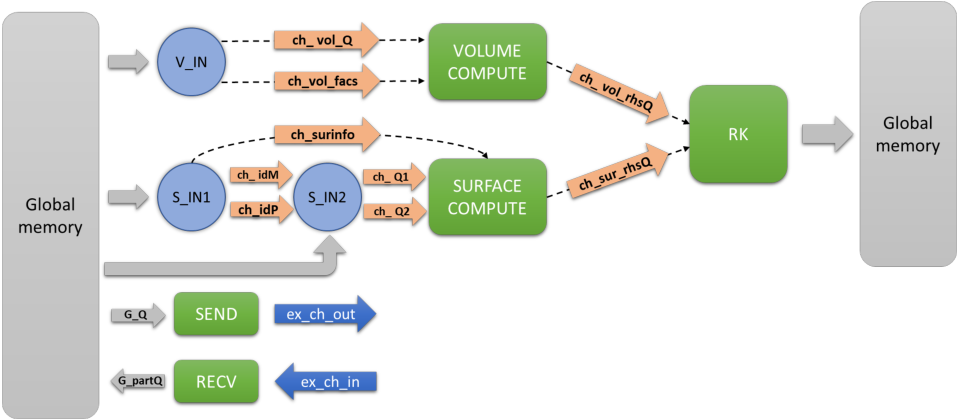
\includegraphics[width=1.0\textwidth]{images/iochan_kernstruc}
    \caption{Structure for \ac{MPI} FPGA OpenCL kernels showing \texttt{send} and \texttt{recv}
    kernels used for communication with external IO channels. Image also shows the internal
    channels introduced between \texttt{VOLUME/SURFACE} to \texttt{RK} kernel}
    \label{fig:iochan_kernstruc}
\end{figure}

In the IO channels design, the computation of shared elements follows the computation of
non-shared elements as in the \texttt{MIDG2 MPI FPGA} design. The major change is the independence of the OpenCL kernels to
communicate the data between the FPGAs without requiring support of the host for
communication. Though host still controls the time step iteration and performs synchronization of kernels between
the computation of non-shared data and the completion of communication of data between two FPGAs.
A comparison of the sequence of operations performed on host and FPGA for the \texttt{MIDG2 MPI FPGA} and
the IO channels design is shown in Figure \ref{fig:sequence_comp}. As the figure shows,
the involvement of the host is decreased. Also due to addition of the channels between
the \texttt{VOLUME/SURFACE} and \texttt{RK} kernel, all kernels in the new design start together instead
of \texttt{RK} following \texttt{VOLUME/SURFACE}.

\begin{figure}[h]
	\centering\small
	\begin{tabular}{l@{\hskip 0.5in}}
        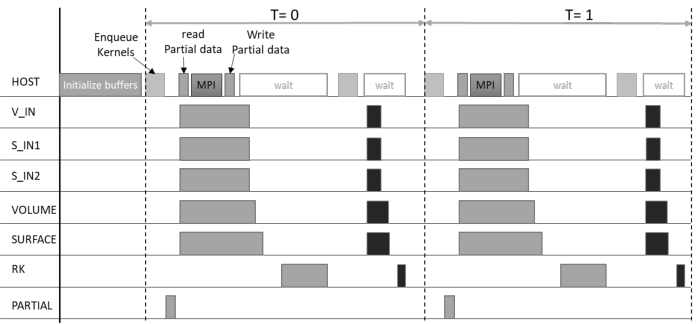
\includegraphics[width=0.8\textwidth]{seq_singlefpga} \\
        \multicolumn{1}{c}{(a) \texttt{MIDG2 MPI FPGA}}  \\
        \\
        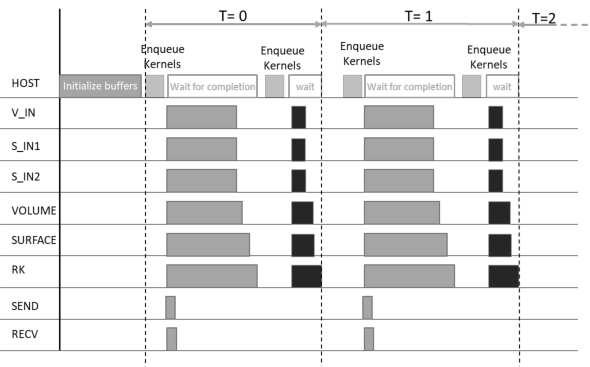
\includegraphics[width=0.7\textwidth]{seq_iochan} \\
        \multicolumn{1}{c}{(b) MIDG2 FPGA with IO channels}
	\end{tabular}
    \caption{Sequence of Kernel and host event for \texttt{MIDG2 MPI FPGA}
    and MIDG2 FPGA with IO channels}
	\label{fig:sequence_comp}
\end{figure}

\section{Host changes to support IO Channels}

The \texttt{host application} of MIDG2 application implements the 3D DG-method introduced in the section \ref{sec:dgtd}.
The application is responsible for following activities:

\begin{itemize}
    \item Read in the mesh and parse the element coordinates and save them in VX, VY and VZ vectors
    \item For a distributed implementation using MPI, partition the mesh using parMETIS library
    and redistribute the elements as per the partition.
    \item Create the information of the shared elements which should be used to identify and map the
    indexes in the field buffer to be shared with the target MPI ranks. The mapping is used to read the
    values and create the partial data buffers to be communicated via MPI or FPGA-to-FPGA link
    \item Perform polynomial interpolation mapping of the geometric element vectors to the standard tetrahedral
    element coordinates using r, s and t values
    \item Compute the geometric coefficients and data layout information (\texttt{vmapM} and \texttt{vmapP})
    \item Setup the OpenCL environment which includes identifying the OpenCL platform and device,
    create OpenCL memory buffers to be used, copy the data to OpenCL memory buffers, program the FPGA with the
    target OpenCL kernel binary and create OpenCL queue to run the kernels.
    \item Run the OpenCL kernels and synchronize the execution over the computed timesteps
    \item Read the results value and compare the analytical and computed results to compute the error
    to estimate the accuracy of the implementation
\end{itemize}

The changes in the host application done mainly are towards enabling the new kernels to function correctly
which involves setting up the OpenCL buffers and control the queueing of the kernels in the correct sequence.
To handle this, the structure of the existing OpenCL platform and device initialization code sections are
updated to handle both the designs with the same host code. A hierarchical structure for the initialization code
is implemented such that, the generic functionalities which include OpenCL platform identification,
context creation etc is separated from the design specific OpenCL buffer
initialization and kernel execution. The new structure of the host code is shown
in Figure \ref{fig:host_appstruc} and would be explained in detail in the section \ref{sec:hostcodeupdate}.

The host application requires an additional json file to get the information about the kernels in the binary such as
the kernel parameter information, dependencies among the kernels and groups of kernels to be executed parallely.
This information is used to configure the kernel buffers as well as setup a execution order tree which is used
to enqueue the kernels in required order and setup other kernel to kernel synchronization using the events.
The main benefit of using the configuration json file is to ease the setup effort for the dependent kernel.
The subgroup structure of the kernels in IO channels design is shown in Listing \ref{code:subgroups}.

\begin{JsonCode}[caption=Kernel subgroups used in Multi FPGA design to enqueue kernels, frame=tlrb, label=code:subgroups]
"kernel_subgroups":
{
    "compute_inner":
    {
        "single_work_item": "true",
        "kernels":
        {
            "maxwell_partial_send":{},
            "maxwell_partial_rcv": {},
            "inputkernel_vol": {},
            "maxwellvolumekernel": {},
            "inputkernel": {},
            "maxwellsurfacekernel": {},
            "inputkernel1": {},
            "maxwellrkkernel": {}
        }
    },
    "compute_halo":
    {
        "single_work_item": "true",
        "kernels":
        {
            "inputkernel_vol": {},
            "maxwellvolumekernel": {},
            "inputkernel": {},
            "maxwellsurfacekernel": {},
            "inputkernel1": {},
            "maxwellrkkernel": {}
        }
    }
}
\end{JsonCode}

The \texttt{compute\_inner} subgroup is responsible for computing the field values for the non-shared
data and perform the data exchange between the FPGAs using the IO channels. As there is no dependencies
listed among any of the kernels in the subgroup, each of the kernels will be executed simultaneously.
The \texttt{compute\_halo} subgroup performs the computation on the shared elements. As the same kernels
are responsible for performing the computation on the shared and non-shared elements, the kernels are
repeated in both the groups. The subgroups help to easily create a execution tree grouping
the same kernels in different groups and order depending upon the implementation which can then be
easily executed on the FPGA device.

Another important modification is done in the host application to get the information about
the mapping of the MPI ranks to the FPGA devices on the node. This mapping is required for the
fully connect topology to setup the correct offsets and number of elements for each of the channels.
The mapping information allows to associate a specific external channel with a MPI rank and hence the
offsets within the \texttt{g\_index} buffer which contains the index values in the \texttt{g\_Q}
buffer for the shared elements. To map the channels, additional information
regarding the MPI rank and associated FPGA device is required. This information is shared using
a structure which contains the MPI host id and associated FPGA device Id which is exchanged
using MPI. After receiving the information about all the ranks, the external channel mapping
is computed locally using a decision tree. The flow chart in Figure \ref{fig:channel_select}
shows the logic of the external channel assignment at each node.
\begin{figure}[ht]%
    \centering
    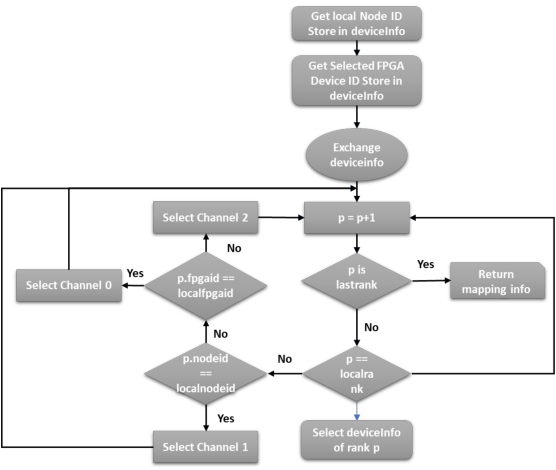
\includegraphics[width=0.7\textwidth]{images/channel_select}
    \caption{Channel selection logic for fully connected topology}
    \label{fig:channel_select}
\end{figure}

